\documentclass[11pt]{article}

\usepackage[margin=1in]{geometry}
\usepackage{amsmath,amssymb}
\usepackage{graphicx}
\usepackage{booktabs}
\usepackage[table]{xcolor}
\usepackage{caption}
\usepackage{hyperref}
\hypersetup{colorlinks=true,linkcolor=blue,citecolor=blue,urlcolor=blue}

\newcommand{\rgnf}{$\rho$-GNF}
\newcommand{\doop}{\mathrm{do}}
\newcommand{\E}{\mathbb{E}}
\newcommand{\N}{\mathcal{N}}

\title{\vspace{-2.5em}A Copula Sensitivity Analysis with $\rho$-GNF:\\
Empirical Study of Treatment-Effect Recovery under Confounding}
\author{Matej Havelka}
\date{\today}

\begin{document}
\maketitle
\vspace{-2em}

\begin{abstract}
\noindent
We study \rgnf{}, a normalizing-flow model that encodes the untestable
no-unobserved-confounding assumption as a single Gaussian-copula parameter $\rho$.
Using synthetic data with a known treatment effect, we ask whether the induced
sensitivity curve behaves sensibly and how accurately the average treatment effect
(ATE) is recovered. When the model is correctly specified the recovery is accurate.
Our main result is a negative one: in a binary-treatment problem, an oracle that is
given the true confounding parameter still recovers the ATE with a seed-to-seed
spread of roughly $40\%$, which is wider than the spread of the biased baselines it
is meant to beat.
\end{abstract}

\section{Causal inference and sensitivity analysis}

Causal inference asks what happens to an outcome $Y$ when we intervene and set a
treatment $A$ to a value $a$, written $\doop(A=a)$~\cite{pearl2009causality}. The
target quantity is the average treatment effect,
\begin{equation}
  \mathrm{ATE} \;=\; \E\!\big[Y \mid \doop(A=1)\big] \;-\; \E\!\big[Y \mid \doop(A=0)\big].
  \label{eq:ate}
\end{equation}
Intervening is not the same as conditioning: in observational data $A$ and $Y$ can
share a common cause, so $\E[Y\mid \doop(A=a)]\neq\E[Y\mid A=a]$ in general. If
every common cause $X$ is observed, the effect is identified under the
unconfoundedness assumption~\cite{imbens2015causal},
\begin{equation}
  \{Y(0),Y(1)\} \perp\!\!\!\perp A \mid X,
  \label{eq:unconf}
\end{equation}
which gives the adjustment formula $\E[Y\mid\doop(A=a)] = \E_X\big[\E[Y\mid A=a, X]\big]$.
Equation~\eqref{eq:unconf} cannot be checked from the data. A hidden confounder $U$
makes it fail and biases any naive estimate.

Sensitivity analysis does not try to verify unconfoundedness. It asks instead how
far the conclusion could move if the assumption failed by a stated
amount~\cite{rosenbaum1983sensitivity}. One picks a scalar $\rho$ that indexes the
strength of the hidden confounding, recomputes the effect as a function
$\mathrm{ATE}(\rho)$, and reports the whole curve rather than a single number. At
$\rho=0$ the estimate coincides with the unconfounded one, and larger $|\rho|$
shows how much confounding would be needed to shrink or reverse the effect.

\section{Copulas and the $\rho$-GNF model}

\paragraph{Copulas.} A copula describes the dependence between two variables
separately from their marginal distributions. By Sklar's
theorem~\cite{nelsen2006copulas}, any joint law of $(A,Y)$ factorises as
$F_{A,Y}(a,y) = C\big(F_A(a),F_Y(y)\big)$, where $F_A,F_Y$ are the marginals and
the copula $C:[0,1]^2\to[0,1]$ carries all the dependence. We use the Gaussian
copula, whose density is
\begin{equation}
  c(u,v;\rho)=\frac{1}{\sqrt{1-\rho^2}}\,
  \exp\!\left(-\frac{\rho^2(\phi_u^2+\phi_v^2)-2\rho\,\phi_u\phi_v}{2(1-\rho^2)}\right),
  \qquad \phi_u=\Phi^{-1}(u),\ \phi_v=\Phi^{-1}(v),
  \label{eq:gausscopdens}
\end{equation}
with a single parameter $\rho\in(-1,1)$. Note that this $\rho$ is the correlation
of the latent normals $\Phi^{-1}(F_A(A))$ and $\Phi^{-1}(F_Y(Y))$; it is not the
Pearson correlation of $A$ and $Y$, and it maps to Kendall's $\tau$ through
$\tau=\tfrac{2}{\pi}\arcsin\rho$. The Gaussian copula also has zero tail
dependence, $\lambda_L=\lambda_U=0$, so it cannot place extra joint mass in a
single tail the way the Clayton or Gumbel families do (Table~\ref{tab:copulas}).
This last point drives the misspecification result in Section~\ref{sec:clayton}.

\begin{table}[h]
\centering
\small
\caption{Dependence properties of the copulas used below. $\lambda_L,\lambda_U$ are
the lower/upper tail-dependence coefficients.}
\label{tab:copulas}
\begin{tabular}{@{}lccc@{}}
\toprule
Family & Kendall's $\tau$ & $\lambda_L$ & $\lambda_U$ \\
\midrule
Gaussian$(\rho)$ & $\tfrac{2}{\pi}\arcsin\rho$ & $0$ & $0$ \\
Clayton$(\theta)$ & $\theta/(\theta+2)$ & $2^{-1/\theta}$ & $0$ \\
Gumbel$(\theta)$  & $1-1/\theta$ & $0$ & $2-2^{1/\theta}$ \\
\bottomrule
\end{tabular}
\end{table}

\paragraph{Graphical normalizing flows.} A normalizing flow is an invertible map
$T_\theta$ that transforms data into simple latent noise and has a tractable
Jacobian, so it can be fitted by maximum likelihood~\cite{papamakarios2017maf}. A
graphical normalizing flow constrains $T_\theta$ to respect a causal
graph~\cite{wehenkel2020gnf}. For the two-variable graph $A\to Y$ we write
$(A,Y)=T_\theta(Z_A,Z_Y)$ with each coordinate map monotone, so $T_\theta$ is a
learned stand-in for the structural mechanisms $A=f_A(Z_A)$ and $Y=f_Y(A,Z_Y)$.

\paragraph{The $\rho$-GNF.} The \rgnf{}~\cite{balgi2024rho} puts the Gaussian
copula on the latent noise,
\begin{equation}
  (Z_A, Z_Y) \sim \N\!\left(\mathbf{0},\,
  \Sigma_\rho = \begin{bmatrix} 1 & \rho \\ \rho & 1 \end{bmatrix}\right).
  \label{eq:copula}
\end{equation}
Because the coordinate maps are strictly increasing, the copula of $(A,Y)$ equals
the copula of $(Z_A,Z_Y)$, so $\rho$ does not change when the marginal shapes of
$A$ and $Y$ change. That invariance is what lets $\rho$ represent the non-causal
association surviving adjustment, i.e.\ the hidden confounding.

To read off an effect we intervene rather than condition. Setting $A=a$ cuts the
arrows into $A$, so the latent link no longer ties $A$ to $Z_Y$ and the outcome
noise keeps its marginal $Z_Y\sim\N(0,1)$. The interventional mean is then
\begin{equation}
  \E[Y\mid \doop(A=a)] \;=\; \E_{Z_Y\sim\N(0,1)}\big[\,g_\theta(a, Z_Y)\,\big],
  \label{eq:invert}
\end{equation}
where $g_\theta=(T_\theta)_Y$ is the fitted outcome map, evaluated by inverting the
flow with the treatment coordinate held at $a$. We estimate the two means in
Eq.~\eqref{eq:ate} by Monte Carlo. Sweeping $\rho$ over $(-1,1)$ and recording
$\mathrm{ATE}(\rho)$ produces the sensitivity curve, which we call the
$\rho$-curve.

\section{Experiments}

All data are synthetic two-variable systems with a known true ATE. We fit the
\rgnf{}, estimate the ATE from Eq.~\eqref{eq:invert}, and report bias and RMSE over
repeated random seeds. Three settings increase the mismatch between model and data:
a Gaussian copula that the model matches exactly (Setting~1), a Clayton copula that
breaks the copula family (Setting~2), and a piecewise-Gaussian system with a binary
treatment where the confounding is fully known (Setting~3).

\subsection{Setting 1: correctly specified Gaussian copula}

The data use a Gaussian copula with true $\rho=0.3$ and true ATE $=0.2$. We hold
the data fixed and vary the assumed $\rho$. Figure~\ref{fig:rho} shows the estimate
moving monotonically through the true value, and the RMSE is smallest at the grid
point nearest the true $\rho$ ($\rho\approx0.26$, RMSE $0.045$).\footnote{The sweep
uses a coarse $20$-point $\rho$-grid and a short training budget, so the located
minimum is limited by the grid resolution rather than found exactly.} This is the
behaviour a sensitivity analysis should have: the correct $\rho$ recovers the
effect, and the curve makes the dependence on that choice explicit.

\begin{figure}[t]
\centering
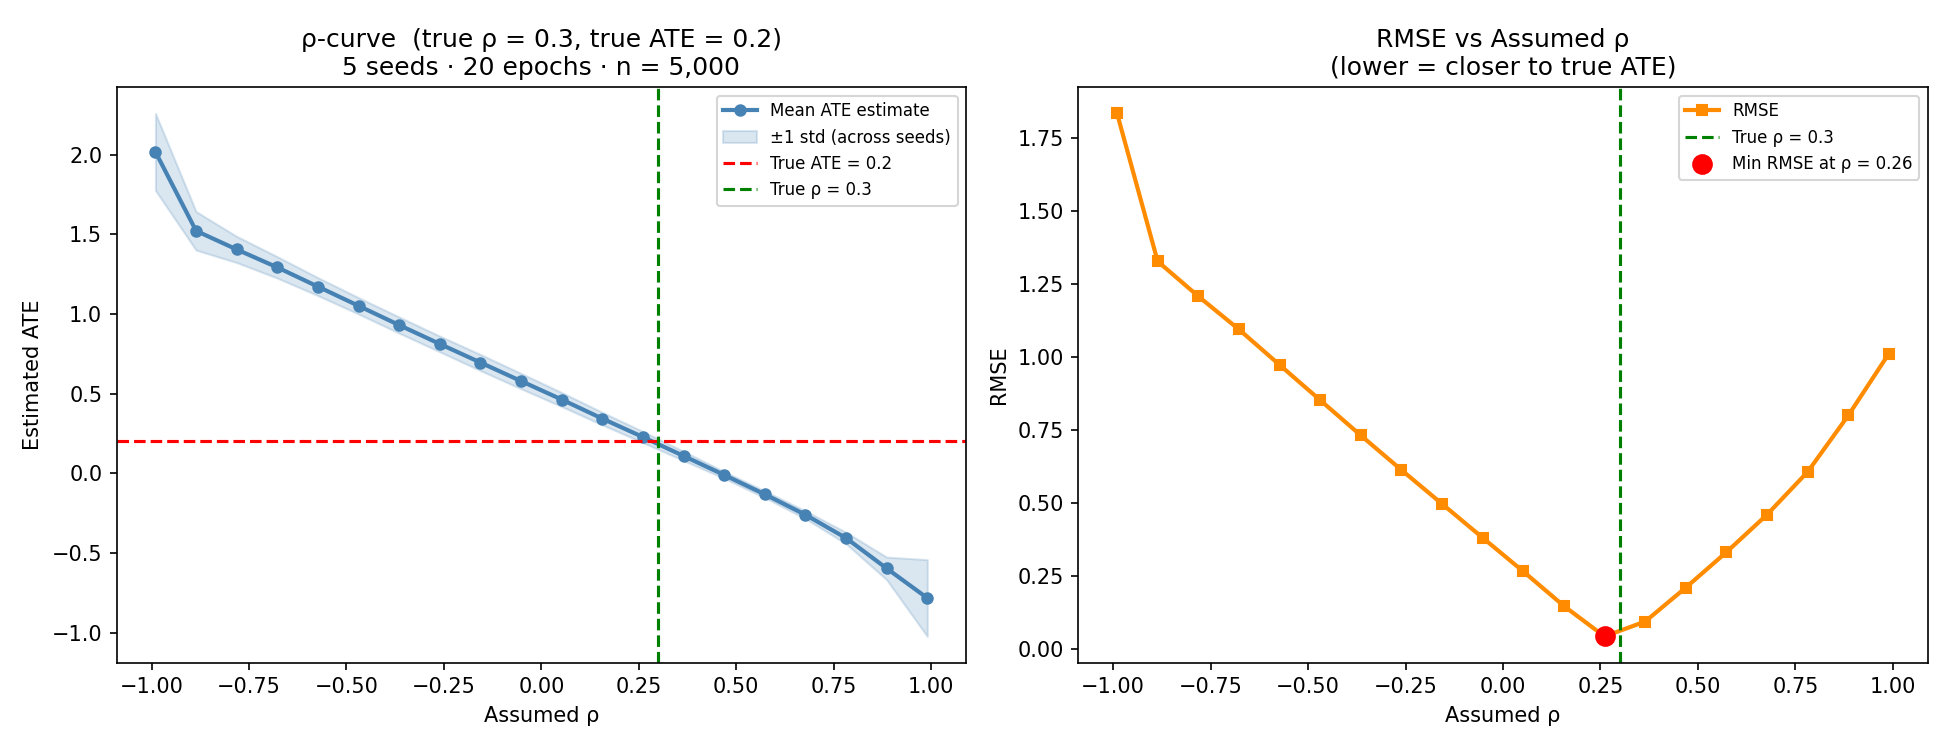
\includegraphics[width=0.88\linewidth]{experiments/results/setting0_rho_sweep/setting0_rho_curve.png}
\caption{Setting 1 $\rho$-curve. Left: mean estimated ATE against assumed $\rho$
(band is $\pm1$ std over seeds); it crosses the true ATE at the true $\rho$. Right:
RMSE against assumed $\rho$, smallest at $\rho\approx0.26$ (true $\rho=0.3$).}
\label{fig:rho}
\end{figure}

\subsection{Setting 2: misspecified copula family (Clayton)}
\label{sec:clayton}

Now the data come from a Clayton copula ($\theta=2$, so $\tau=0.5$) with
standard-normal margins, while the model still assumes a Gaussian copula. Matching
the two families on rank correlation gives the reference value
$\rho_{\mathrm{ref}}=\sin(\pi\tau/2)\approx0.707$. In the sweep, however, the
RMSE-minimising assumed $\rho$ is about $0.33$, well below $\rho_{\mathrm{ref}}$,
and the bias grows with the size of the true effect. The explanation is tail
dependence. Clayton has $\lambda_L=2^{-1/2}\approx0.71$, so treatment and outcome
move together in the lower tail, whereas the Gaussian copula forces
$\lambda_L=0$. No single $\rho$ can reproduce both the bulk rank correlation and the
tail behaviour at once, so the $\tau$-matched value is not the one that best
recovers the effect. Choosing $\rho$ from $\tau$ alone can therefore mislead when
the true copula is not Gaussian.

\subsection{Setting 3: binary treatment with known confounding}

This setting is deliberately simple and the confounding is fully specified:
\begin{equation*}
  X\sim\mathrm{U}(-1,1),\quad
  Z_Y\mid Z_A,X \sim \N\!\big(\rho(X)Z_A,\,1-\rho(X)^2\big),\quad
  \rho(X)=\begin{cases}-0.5 & X<0\\ \phantom{-}0.8 & X\ge0,\end{cases}
\end{equation*}
with $A=\mathrm{Bernoulli}\big(\sigma(X+Z_A)\big)$ and $Y=Z_Y+\mathrm{ATE}\cdot A$,
true ATE $=1$. The observed confounder $X$ shifts both the treatment propensity
$\sigma(X+Z_A)$ and the latent correlation $\rho(X)$. We compare two misspecified
constant-$\rho$ models against a split-$\rho$ oracle that fits a separate fixed-$\rho$
flow on each stratum $X<0$ and $X\ge0$ using the true $\rho(X)$.

Over $20$ seeds with $n=10{,}000$ the oracle is almost unbiased on average
($0.940$ against a true $1.0$), yet its estimates range from $0.59$ to $1.38$
across seeds, a spread of about $\pm40\%$. Its standard deviation, $0.210$, is
roughly three times that of either biased baseline, and its RMSE is the largest of
the three (Table~\ref{tab:piecewise}, Figure~\ref{fig:piecewise}).

Why does the correct model estimate so poorly on a single dataset? The treatment is
binary and the propensity $\sigma(X+Z_A)$ can sit close to $0$ or $1$, so overlap
(positivity) is weak and the $\doop(A=1)$ versus $\doop(A=0)$ contrast leans on
sparsely sampled regions of the latent space. The oracle then splits the sample by
the sign of $X$, leaving about $n/2$ points to fit each flow, which inflates the
Monte-Carlo and estimation variance further. Using the correct $\rho(X)$ removes the
bias but does nothing about this variance.

\begin{table}[t]
\centering
\small
\caption{Binary-treatment piecewise copula, $20$ seeds, true ATE $=1$. The oracle
is the least biased but has the widest spread and the worst RMSE. The highlighted
row is the oracle.}
\label{tab:piecewise}
\begin{tabular}{@{}lrrrrr@{}}
\toprule
Variant & mean & std & min--max (range) & bias & RMSE \\
\midrule
fixed $\rho=0$ (misspec.)    & $1.116$ & $0.078$ & $0.97$--$1.29$ ($0.32$) & $+0.116$ & $0.140$ \\
fixed $\rho=0.15$ (misspec.) & $0.865$ & $0.073$ & $0.72$--$1.01$ ($0.29$) & $-0.135$ & $0.154$ \\
\rowcolor{gray!15}
split-$\rho$ oracle (true)   & $0.940$ & $0.210$ & $0.59$--$1.38$ ($0.79$) & $-0.060$ & $0.219$ \\
\bottomrule
\end{tabular}
\end{table}

\begin{figure}[t]
\centering
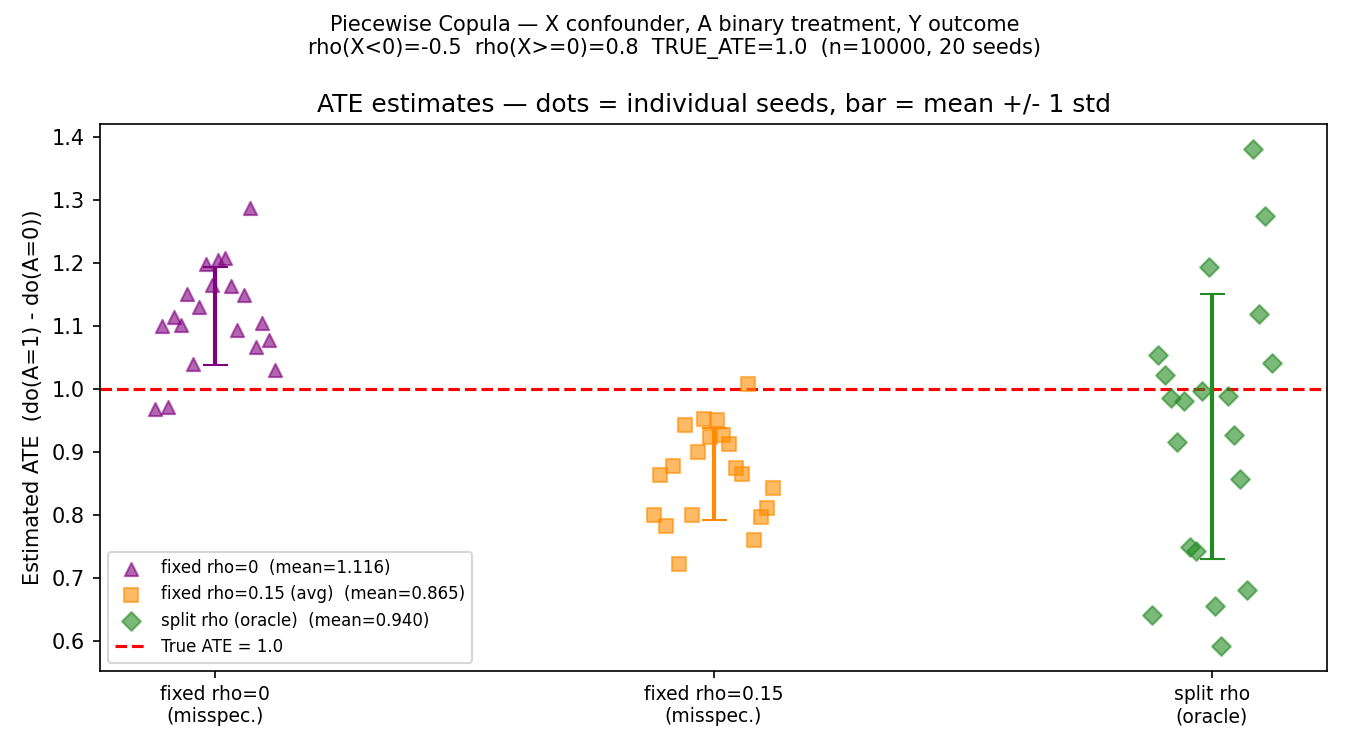
\includegraphics[width=0.66\linewidth]{experiments/results/setting_piecewise_copula/ate_figure.png}
\caption{Binary-treatment piecewise copula. Dots are individual seeds, bars are
mean $\pm1$ std, and the dashed red line is the true ATE. The oracle (green), given
the true $\rho(X)$, scatters much more widely than the biased constant-$\rho$
baselines.}
\label{fig:piecewise}
\end{figure}

\section{Conclusion}

The \rgnf{} gives a usable copula sensitivity analysis. When $\rho$ is chosen well
the $\rho$-curve passes through the true effect and shows how the conclusion depends
on the unverifiable confounding assumption. The experiments also expose two limits.
Under a misspecified copula family the best assumed $\rho$ is not the value that
matches rank correlation, because the Gaussian copula cannot reproduce tail
dependence. And a correct sensitivity parameter does not by itself buy a reliable
estimate: for a binary treatment the oracle still scatters by about $\pm40\%$ across
datasets, driven by weak overlap and the reduced sample per stratum. In practice one
should report the $\rho$-curve together with a variance estimate from repeated fits,
not a single number. The main caveat of this study is its scale. The sweeps use a
coarse $\rho$-grid and a short training budget, and every setting is a synthetic
two-variable system, so the numbers are indicative rather than tuned.

{\small
\bibliographystyle{plain}
\bibliography{ref}
}

\end{document}
